\subsection{Literature Review}
In order to carry out the study and develop the tool needed for studying drivers' behaviour, a non-exhaustive literature and resource study was carried out regarding state of the art and current resources available to the team.

% \subsubsection{Driver Models}
% Driver models serve as an important input in predicting driver reaction and developing active safety systems. Computational driver models define specific decisions based on previous information in order to carry out a task. Those decisions are translated into computations that the driver system follows \cite{CompDrivMod}. Such models can, for example, be used for the assessment of predictive safety benefits and for the definition of warning strategies. These are used to predict human behaviour in different critical scenarios, and act upon these predictions to mitigate or reduce the severity of crashes.

% There are different driver models with different complexities. One well known model is the 
% car following model presented by Gazis, Herman, and
% Rothery (1961). In this model the diver aims to keep the same speed as the  lead vehicle, and corrects to speed changes faster at higher speed, low headway distances . Parameters for this model were tuned through conducting follow the lead experiments \cite{bexelius1968extended}. This model was later extended to account for a number of error inducing driver behaviours and stochasticity and have been used for evaluating active safety systems, such as FCW \cite{markkula2012review}.




\subsubsection{Camera model and rectification}
To be able to carry out image processing techniques on images, one would first have to determine a camera model and rectify the images in hand for distortions and camera pose. As seen over the years, the pinhole camera model is the most generic camera model used. The theory behind the pinhole camera model is described in details in \cite{xu2013epipolar}. This popular camera model has proven to be a reliable model in several applications such as in close-range \cite{duane1971close} or wide-angle lenses \cite{swaminathan2000nonmetric}. Figure \ref{fig:pinhole_model} shows a basic simplified  pinhole camera model.

\begin{figure}[H]
    \centering
    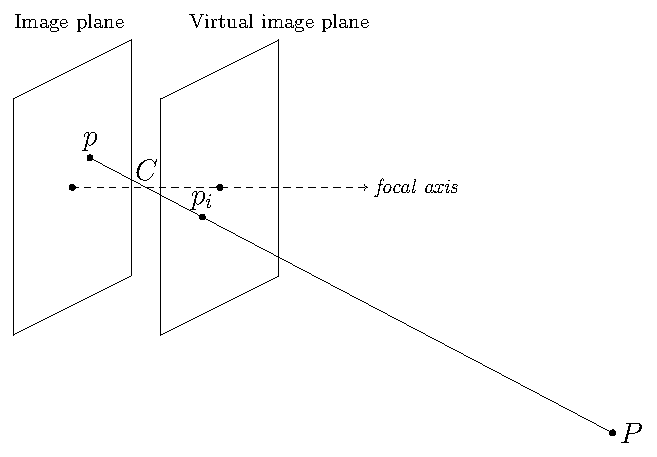
\includegraphics[width = 0.6\textwidth]{Figures/camera_model_1.pdf}
    \caption{Pinhole Camera Model}
    \label{fig:pinhole_model}
\end{figure}

Camera calibration and image rectification are well studied subjects and are becoming  more important with the increasing need for higher accuracy measurement in computer vision. For geometrical measurements, the main concern is camera distortion \cite{wang2008new}.

Radial distortion causes an inward or outward displacement of a given image point from its ideal location while tangential distortion causes a rotational displacement about the center of the image. These effects are better explained with figures in \cite{wang2008new}. These distortions are caused by either the spherical shape or the position of the camera lens and results in straight objects in reality to appear curved in the image. Image rectification is therefore needed to get a better estimation of the real world position of objects in an image.

There are two sets of parameters that are needed for image rectification, these are internal (intrinsic) and external (extrinsic)  camera parameters. Internal parameters determine the image coordinates of a point given the spatial position of said point with respect to the camera. External parameters characterise the geometrical relation between the camera and the scene \cite{wang2008new}. While intrinsic calibration is only done once for a camera, extrinsic calibration is required when the position and orientation of the camera is subjected to large changes, such as the case of a vehicle driving on the road \cite{wang2004simple}. Given a sufficient number of visible points, their placement in the image, and their placement in real world coordinates, the internal and external camera parameters can be estimated \cite{wang2008new}.




\subsubsection{Lane detection}

Lane detection is a crucial part of the development of autonomous vehicles and many active safety systems, such as Lane Keep Assist (LKA), Lane Departure Warning (LDW) and Lane Change Support (LCS). In these applications, lanes are in most cases detected in real-time with computer vision technologies, by using one or multiply road facing cameras mounted at the front of a vehicle. Lane detection is also used to analyse NDS videos in order to extract information about the events that lead to a crash or a near-crash \cite{IEEE2014}. In fact, lane change events, lane type and vehicle localisation using lanes are some of the most important measures when it comes to investigation of crash and pre-crash events \cite{IEEE2014}. The goal of this literature review is to investigate how a lane detection algorithm can be structured and how it can be used in practice.

\paragraph{Algorithm}
A simple but robust lane detection algorithm is described in \cite{Compvision}. The input data to the algorithm is an image captured by a road-facing camera mounted on a moving vehicle. In order to detect the lanes, the image needs to be processed. The basic idea behind lane detection is to identify the lane boundaries, or the edges of the lanes. The edges of the lane can be defined as a rapid change in intensity from one pixel to another. In the case of detecting the lanes on a road, the difference in intensity between the yellow or white lane and the gray asphalt needs to be identified \cite{EdgeDet}. In order to easier detect change in colour, the image in the algorithm \cite{Compvision} is converted to grayscale. An alternative approach is to filter out all the colours in the image except for yellow and white and therefore distinguish the lanes from other objects in the image. The problem with this approach is that worn out lanes have a different colour than newer lanes, and the brightness of the image affects the colour,  making it hard to find a colour threshold which will work in all videos \cite{ColorScale}. The next step in the construction process of the algorithm described in \cite{Compvision} is to remove noise from the image, for example strong shadows. One of the most used filters in these kinds of tasks is the Gaussian blur filters, which is a low pass filter that smoothens the image \cite{GaussianFilter}. There are also filters that adjust the brightness and contrast of the image. The contrast between the asphalt and the lane is identified by using an edge detector.

For the algorithm described in \cite{Compvision}, a canny edge detector was used. In order to determine which of the identified edges are lanes, the algorithm \cite{Compvision} used a Hough transform to search for lines which are horizontal with a maximum of 45 degrees slope to either the left or the right. These identified lines are considered lanes, all the other detected lines are rejected. The last step in the development process of the algorithm described in \cite{Compvision} is to define the region of interest (ROI).  In this step, the processed image is cropped so all unnecessary information in the image is rejected, for example the environment on the side of the road. In this case, ROI only consist of the road near the vehicle.

\paragraph{Critical aspects} 
Even though lane detection methods have been improved during recent years, there are still challenges to overcome in this field. Complex illuminations and shadows from the environment can cause the camera to miss lanes on the road, or wrongly recognise objects and shadows as lanes \cite{Compvision}. The ability of the algorithms to detect lanes is heavily dependent on the time of the day, the weather and the season of the year. In order for the lane detection algorithm to be robust, it must be able to detect the lanes in different conditions.

\subsubsection{Heading angle and lateral offset estimation}
Calculating the heading angle of the POV is not an easy task, especially using a mono camera system. 

In \cite{3dtrajectory}, the authors estimate the 3D pose of an object by following some feature points between frames and constructing a 3D trajectory as well as the object's structure. The estimation is fortified by using the optical flow of the feature points. A more straightforward method is introduced in \cite{realtimePoseEstimation} where an extended Kalman filter is used to estimate the rotation and translation of an object between frames, given that the feature points' coordinates are known in 3D-space and 2D-space.

Another method, proposed in \cite{FeatureBasedHomography}, utilises the concept of homography for calculating the change in a plane between frames. This method was intended to calculate the angular rate of a POV along intersections and curves. The calculation is enhanced using an extended Kalman filter to better track feature points between frames. The homography method is also utilized in \cite{UAVPoseEstimation} to estimate the yaw angle of an unmanned aerial vehicle (UAV). The proposed method uses a reference on the ground to calculate the homographies over time and estimate the yaw angle from that.

Finally, a method is developed by Nilsson where the heading angle of the POV is estimated by measuring the POV corners in relation to its previously known length and width \cite{nilsson2018}. This method was found to be reliable on proper measurements which can sometimes not be available based on the quality of the frames taken by the camera, in addition to the prior estimation of the POV's width and length.

\subsubsection{Range and range rate estimation}
Intelligent vehicle systems are increasingly relying on vehicle sensors for calculation of distances and speeds between vehicles \cite{IVSsurvey}. Engineers have used different sensors and hardware for range estimation and speed calculation. Some of those vehicular systems used for range estimation are radars, lidars and camera systems, being monocular and stereo vision used for distance calculation \cite{radarLidarCamera}. In fact, radars can also provide a range rate estimation using the Doppler effect \cite{radarDoppler}. Time-of-flight cameras are also an option for distance calculation that offers depth scanning of the environment as well \cite{timeofflightcam}.

For the distance estimation using a monocular vision camera, several methods have been developed. One of those methods would be using the width of a vehicle and its corresponding number of pixels in the image frame \cite{nilsson2018}. Another method suggested machine learning for 3D reconstruction using a still monocular camera setup \cite{Saxena2008}. Several research has also been conducted on distance calculation using the triangulation method with accounting for the pitch angle of the camera as in \cite{triangulation1}, \cite{alizadeh2015object} and \cite{triangulation2}. An interesting approach that is based on the triangulation method and takes into account the extrinsic parameters of the camera (pitch, yaw and roll) is discussed in \cite{SLee2012}: the authors define a homography matrix that rotates the image in such a way that the camera in the rotated image is pointing towards the vanishing point of the lanes. This homography matrix is based on the Euler-Rodrigues rotation formula \cite{Palais2007}. The optical flow method is also one option for measuring the motion of an object between frames by the tracking of feature points \cite{meng2016tool}.

\subsubsection{Manual Annotation}

Manual annotation for extracting data from videos can be a time- and resource-consuming task \cite{schreiner2007semi}. Since SHRP2 does not include data about the lead vehicle, such as lateral speed, longitudinal speed and lateral position in the lane, this data is currently acquired through manual annotation of the videos, where the annotator manually measures the pixel width of the lead vehicle in the image with a ruler and a constant assumed vehicle width \cite{bargman2013using}. 

Environmental factors, such as surface condition, lighting condition, forward visibility are also identified using the forward roadway view footage \cite{hallmark2015evaluation}. 

For studying safety-critical lane changes, one study was found that used dash-cam footage from the SV. Annotation in this study was done through viewing the video and noting the time where half of the SV has crossed the lane edge \cite{beggiato2013sequence}.

In an other study, \textit{comprehensive Examination of Naturalistic Lane-Changes}, a population of 8,667 lane changes were studied. This population was constructed using two research vehicles driven by 16 participants over the period of 320 days. The vehicles used in this study were modified and equipped with radars and cameras on all sides of the vehicles enabling full comprehension of the SV's surroundings. A Sample of 500 critical lane changes was chosen for an in-depth analysis. A tool was used to integrate video, radar and sensor data to display the event in a graphical representation. The tool allowed the annotator to study the behaviour of the driver during the lane-changing manoeuvre using the driver face camera. It also allowed the annotator to estimate the curvature of the lanes through using sliders and a comparison to the video image \cite{lee2004comprehensive}. 

% \textcolor{red}{This part needs to be expanded \cite{lee2004comprehensive} and \cite{beggiato2013sequence} are sources}


\subsubsection{Python Modules}

Python offers the ability to use numerous open source modules and libraries for different computer vision applications. Below is a brief description of some of those  modules and libraries. A more detailed description of the exact versions used in the project environment is included in the appendix.

\subsubsection*{OpenCV}

The openCV library is an open source tool that provides many image processing functions \cite{OpenCV}. One of its functionalities is that it can read images from a video file frame by frame and display said images in a predefined window. It can also, in the same window, edit the image with multiple drawing functions using the keyboard and mouse as inputs. There are also some image recognition tools that can be helpful for the future automatization of the annotation tool.

% The tool is capable of reading images and displaying them into a window, and can edit the image with multiple draw functions using the mouse and keyboard as input. 


\subsubsection*{Numpy}

This is a general purpose array processing package that provides high-performance multidimensional array objects and tools for working for these arrays \cite{numpy_module}.

% This is helpful in this project since images and user inputs are stored in arrays. The tools that Numpy provides therefore used in many functions that handle image processing and data interpolation. 

\subsubsection*{Scipy}

Scipy is a scientific library that has functions to import and export data to and from $.mat$ files in Python \cite{scipy_module}.

\subsubsection*{Math}

The Python Math library offers access to some common math functions and constants in Python \cite{math_module}. This library is a built-in module in Python, hence needs no installation. It does, however, require to be imported in the script where its functions are to be used.  

\subsubsection*{Tkinter}

Tkinter is the most commonly used GUI programming toolkit for Python and therefore has many tutorials on how to make a simple GUI \cite{Tkinter_module}. 

\subsubsection*{Pickle}

Python's Pickle module is used for serializing and de-serializing a Python object structure. Any object in Python can be pickled so that it can be saved on disk. What Pickle does is that it “serializes” the object first before writing it to file. Pickling is a way to convert a python object (list, dict, etc.) into a character stream. The idea is that this character stream contains all the information necessary to reconstruct the object in another python script \cite{Pickle_module}.

\subsubsection*{Matplotlib}

The Matplotlib is a Python 2D plotting library that is easy to use and produces publication quality figures \cite{matplotlib}.

\subsubsection*{Time}

The time module contains several time relate functions \cite{Time_module}.


